\chapter{Recursive Value Definitions: The Fixrec Package}
\label{ch:fixrec}

\section{Introduction}

In Haskell and most other functional programming languages, recursive definitions are supported directly: In the definition of a function, the constant being defined may occur freely on the right-hand side. This is in contrast to a theorem prover like Isabelle, whose primitive definitions are required to be non-recursive in order to guarantee logical soundness.

In Isabelle, a recursive specification of a new constant cannot be used directly as a definition. The specification must be used indirectly: First, the recursive specification must be somehow transformed into a \emph{non}-recursive definition of the constant. Second, this definition can then be used to prove the original specification as a theorem.

Isabelle/HOL already includes a number of packages that mechanize this kind of process for certain kinds of recursive definitions. The \textsc{Datatype} package provides the \isa{primrec} command for defining primitive-recursive functions over data\-types \cite{isabelle-tutorial}; the \textsc{Recdef} and \textsc{Function} packages define functions that use well-founded recursion \cite{Slind96recdef, Krauss10a}.

In \HOLCF{99}, no definition package for general recursive functions existed; such functions could only be defined by explicitly using the domain-theoretic fixed point combinator \isa{fix}. Users had to derive recursive equations manually, using the theory of least fixed points. This chapter introduces the {\fixrec} package for Isabelle/HOLCF, which automates this process: Users of \HOLCF{11} can now use {\fixrec} to formalize Haskell-style recursive function definitions directly.

\paragraph{Contributions.} The current implementation of \textsc{Fixrec} derives from the original version by Amber Telfer in 2004~\cite{Telfer04}. Since then, many new features have been added by the present author: The current version supports mutual recursion, and curried functions with any number of arguments. It also supports a wider class of patterns: Function definitions can use lazy or strict constructors, including constructors from Isabelle/HOL datatypes; definitions with overlapping patterns are also supported. The package is now suitable for verifying real Haskell programs: Some example case studies using \textsc{Fixrec}, including proofs by least fixed point induction, can be found in Chapter~\ref{ch:case-domain}.

\paragraph{Overview.} The remainder of this chapter starts by describing the features of the {\fixrec} package, from a user's point of view (\S\ref{sec:fixrec-features}). Then we establish an implementation strategy, showing how to translate lists of function equations into non-recursive definitions by expressing recursion with a fixed point combinator (\S\ref{sec:fixrec-fix}) and performing pattern match compilation (\S\ref{sec:fixrec-match}). Next are details of the actual implementation of the {\fixrec} package (\S\ref{sec:fixrec-impl}). Finally, we conclude with a comparison to related work, and directions for future work (\S\ref{sec:fixrec-conclusion}).

\section{Fixrec package features}
\label{sec:fixrec-features}

The {\fixrec} package lets users define recursive functions and values in HOLCF much like they can in Haskell or ML. Users can write function specifications with patterns, involving datatypes that may have been defined by the user. Users can use recursion freely within groups of simultaneously-defined values, with no need for termination proofs. The {\fixrec} package generates definitions for constants, proves each defining equation as a theorem, and also generates induction rules for reasoning about the new constants.

Patterns in \textsc{Fixrec} definitions can mention any of the constructors for basic HOLCF types (\S\ref{sec:holcf-types}): \isa{spair}, \isa{sinl}, \isa{sinr}, \isa{up}, \isa{ONE}, \isa{TT}, \isa{FF}, and also the \isa{Pair} constructor \isa{(_, _)} from Isabelle/HOL. Constructors for types defined by the \textsc{Domain} package are also supported, for instance \isa{LNil} and \isa{LCons} from the lazy list type below.
%
\indexdefx{domain 'a llist}
\indexdefx{LNil}
\indexdefx{LCons}
\begin{isacode}
domain 'a llist = LNil | LCons (lazy "'a") (lazy "'a llist")
\end{isacode}

The syntax for the \isa{fixrec} command is similar to other definition commands like \isa{primrec} or the \textsc{Function} package's \isa{fun} command. (A full syntax diagram is shown in Fig.~\ref{fig:fixrec-syntax}.) The equations must be separated by vertical bars; theorem names for each equation are optional.
%
\indexdefx{firsts}
\indexthmx{firsts_LNil}
\indexthmx{firsts_LCons}
\begin{isacode}
fixrec firsts :: "('a \<times> 'b) llist -> 'a llist"
  where firsts_LNil: "firsts`LNil = LNil"
  | firsts_LCons: "firsts`(LCons`(x, y)`xs) = LCons`x`(firsts`xs)"
\end{isacode}
%
The definition above generates the theorems \isa{firsts_LNil} and \isa{firsts_LCons}. It also declares a theorem list \isa{firsts.simps} consisting of all equations in the definition; these are added to the simplifier by default.

%%%%%%%%%%%%%%%%%%%%%%%%%%%%%%%%%%%%%%%%%%%%%%%%%%%%%%%%%%%%%%%%%%%%%%
\begin{figure}
\begin{center}
\begin{minipage}{0.625\linewidth}

\emph{definition}:

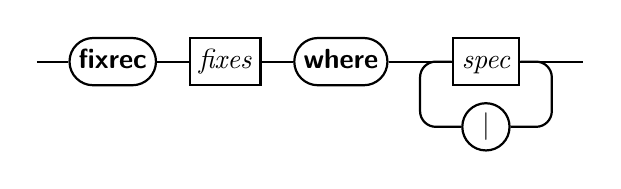
\begin{tikzpicture}
[ thick, draw, text height=1.5ex, text depth=0.4ex
, point/.style={coordinate}
, keyword/.style={rectangle, minimum size=6mm, rounded corners=3mm, draw, font=\bfseries\sffamily}
, terminal/.style={rectangle, minimum size=6mm, rounded corners=3mm, draw, font=\sffamily}
, nonterminal/.style={rectangle, minimum size=6mm, draw, font=\itshape}
, curve/.style={rounded corners=2mm}
]
\matrix[row sep=2mm, column sep=4mm] { 
% First row: 
\node (p0) [point] {}; &
\node (fixrec) [keyword] {fixrec}; & 
\node (fixes) [nonterminal] {fixes}; & 
\node (where) [keyword] {where}; & 
\node (p1) [point] {}; &
\node (spec) [nonterminal] {spec}; &
\node (p2) [point] {}; &
\node (p3) [point] {}; \\ 
% Second row: 
& & & & & \node (bar) [terminal] {\textbar}; & & \\ 
};
\draw [curve] (spec) -- (p2) |- (bar) -| (p1) -- (spec);
\draw [curve] (p0) -- (fixrec) -- (fixes) -- (where) -- (spec) -- (p3);
\end{tikzpicture}

\emph{fixes}:

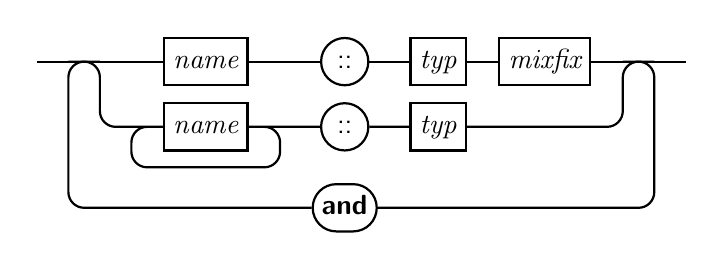
\begin{tikzpicture}
[ thick, draw, text height=1.5ex, text depth=0.4ex
, point/.style={coordinate}
, keyword/.style={rectangle, minimum size=6mm, rounded corners=3mm, draw, font=\bfseries\sffamily}
, terminal/.style={rectangle, minimum size=6mm, rounded corners=3mm, draw, font=\sffamily}
, nonterminal/.style={rectangle, minimum size=6mm, draw, font=\itshape}
, curve/.style={rounded corners=2mm}
]
\matrix[row sep=2mm, column sep=4mm] { 
% First row:
\node (p0) [point] {}; &
\node (p1) [point] {}; &
\node (p2) [point] {}; & &
\node (bind1) [nonterminal] {name}; & &
\node (colon1) [terminal] {::}; &
\node (typ1) [nonterminal] {typ}; &
\node (mixfix) [nonterminal] {mixfix}; &
\node (p3) [point] {}; &
\node (p4) [point] {}; &
\node (p5) [point] {}; \\
% Second row:
& & &
\node (p6) [point] {}; &
\node (bind2) [nonterminal] {name}; &
\node (p7) [point] {}; &
\node (colon2) [terminal] {::}; &
\node (typ2) [nonterminal] {typ}; \\
% Third row:
& & & &
\node (p8) [point] {}; \\
% Fourth row:
& & & & & &
\node (and) [keyword] {and}; \\
};
\draw [curve] (p0) -- (p1) -- (p2) -- (bind1) -- (colon1) -- (typ1) -- (mixfix) -- (p3) -- (p4) -- (p5);
\draw [curve] (p1) -- (p2) |- (bind2) -- (p7) |- (p8) -| (p6) -- (bind2) -- (colon2) -- (typ2) -| (p3) -- (p4);
\draw [curve] (p3) -- (p4) |- (and) -| (p1) -- (p2);
\end{tikzpicture}

\emph{spec}:

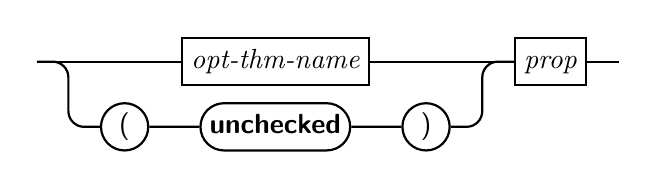
\begin{tikzpicture}
[ thick, draw, text height=1.5ex, text depth=0.4ex
, point/.style={coordinate}
, keyword/.style={rectangle, minimum size=6mm, rounded corners=3mm, draw, font=\bfseries\sffamily}
, terminal/.style={rectangle, minimum size=6mm, rounded corners=3mm, draw, font=\sffamily}
, nonterminal/.style={rectangle, minimum size=6mm, draw, font=\itshape}
, curve/.style={rounded corners=2mm}
]
\matrix[row sep=2mm, column sep=4mm] { 
% First row:
\node (p0) [point] {}; &
\node (p1) [point] {}; & &
\node (name) [nonterminal] {opt-thm-name}; & &
\node (p2) [point] {}; &
\node (prop) [nonterminal] {prop}; &
\node (p3) [point] {}; \\
% Second row:
& &
\node (lparen) [terminal] {(}; & 
\node (unchecked) [keyword] {unchecked}; & 
\node (rparen) [terminal] {)}; & & & \\
};
\draw [curve] (p0) -- (p1) -- (name) -- (p2) -- (prop) -- (p3);
\draw [curve] (p0) -- (p1) |- (lparen) -- (unchecked) -- (rparen) -| (p2) -- (prop);
\end{tikzpicture}

\emph{opt-thm-name}:

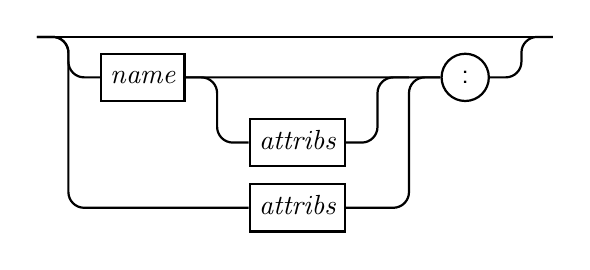
\begin{tikzpicture}
[ thick, draw, text height=1.5ex, text depth=0.4ex
, point/.style={coordinate}
, keyword/.style={rectangle, minimum size=6mm, rounded corners=3mm, draw, font=\bfseries\sffamily}
, terminal/.style={rectangle, minimum size=6mm, rounded corners=3mm, draw, font=\sffamily}
, nonterminal/.style={rectangle, minimum size=6mm, draw, font=\itshape}
, curve/.style={rounded corners=2mm}
]
\matrix[row sep=2mm, column sep=4mm] { 
% First row:
\node (p0) [point] {}; &
\node (p1) [point] {}; & & & & & & &
\node (p2) [point] {}; &
\node (p3) [point] {}; \\
% Second row:
& &
\node (name) [nonterminal] {name}; &
\node (p4) [point] {}; & &
\node (p5) [point] {}; &
\node (p6) [point] {}; &
\node (colon) [terminal] {:}; \\
% Third row:
& & & &
\node (attribs1) [nonterminal] {attribs}; \\
% Fourth row:
& & & &
\node (attribs2) [nonterminal] {attribs}; \\
};
\draw [curve] (p0) -- (p1) -- (p2) -- (p3);
\draw [curve] (p0) -- (p1) |- (name) -- (colon) -| (p2) -- (p3);
\draw [curve] (name) -- (p4) |- (attribs1) -| (p5) -- (p6);
\draw [curve] (p0) -- (p1) |- (attribs2) -| (p6) -- (colon);
\end{tikzpicture}

\end{minipage}
\end{center}

\caption{Input syntax for {\fixrec} package}
\label{fig:fixrec-syntax}
\end{figure}
%%%%%%%%%%%%%%%%%%%%%%%%%%%%%%%%%%%%%%%%%%%%%%%%%%%%%%%%%%%%%%%%%%%%%%

\paragraph{Lazy and strict constructors.} The {\fixrec} package works best with lazy constructor functions like \isa{LCons}, \isa{Pair} and \isa{up}. It also works with strict constructor functions, but definedness side conditions like \isa{x ~= \<bottom>} may be required.
%
\indexdefx{from_sinl}
\begin{isacode}
fixrec from_sinl :: "'a \<oplus> 'b -> 'a"
  where "x ~= \<bottom> ==> from_sinl`(sinl`x) = x"
\end{isacode}
%
If the side-condition in the above definition is omitted, the {\fixrec} package will not be able to prove the equation, and it will fail with an error message. Note that combinations of strict and lazy constructors can avoid the need for such side conditions.
%
\indexdefx{from_sinl_up}
\begin{isacode}
fixrec from_sinl_up :: "'a\<lifted> \<oplus> 'b -> 'a"
  where "from_sinl_up`(sinl`(up`x)) = x"
\end{isacode}
%
Even though \isa{sinl} is a strict constructor, the side condition \isa{up`x /= UU} is not needed. This is because \isa{up} is a lazy constructor and {\fixrec} can determine \isa{up`x /= UU} automatically.

\paragraph{Overlapping patterns.} The {\fixrec} package supports definitions with overlapping patterns. For example, consider the following function that zips two lists together: The first equation has specific patterns, while the second equation is a catch-all default case. The second equation cannot be proved as a theorem because it only applies when the first pattern fails.
%
\indexdefx{lzip}
\begin{isacode}
fixrec lzip :: "'a llist -> 'b llist -> ('a \<times> 'b) llist"
  where "lzip`(LCons`x`xs)`(LCons`y`ys) = LCons`(x, y)`(lzip`xs`ys)"
  | (unchecked) "lzip`xs`ys = LNil"
\end{isacode}
%
Usually {\fixrec} tries to prove all equations as theorems. The \isa{unchecked} option overrides this behavior, so {\fixrec} does not attempt to prove that particular equation. With the \isa{lzip} example, both equations influence the definition of \isa{lzip}, but only the first is proved as a theorem. The generated theorem list \isa{lzip.simps} then consists of only the first equation.

\paragraph{Generating extra equations.} The {\fixrec} package provides automation for proving extra equations beyond those included in the function definition. This takes the form of a proof method called \isa{fixrec_simp}. One use for \isa{fixrec_simp} is to prove specific rules for functions defined with overlapping patterns, like our earlier example \isa{lzip}.
%
\indexthmx{lzip_extra_simps}
\begin{isacode}
lemma lzip_extra_simps [simp]:
  shows "lzip`(LCons`x`xs)`LNil = LNil" and "lzip`LNil`ys = LNil"
  by fixrec_simp+
\end{isacode}
%
Another common use of the \isa{fixrec_simp} method is to prove strictness rules for functions.
%
\indexthmx{lzip_strict}
\begin{isacode}
lemma lzip_strict [simp]:
  shows "lzip`\<bottom>`ys = \<bottom>" and "lzip`(LCons`x`xs)`\<bottom> = \<bottom>"
  by fixrec_simp+
\end{isacode}
%
Functions defined by {\fixrec} satisfy the same strictness properties that we would find in Haskell, according to a left-to-right pattern matching strategy. For example, \isa{lzip`\<bottom>`LNil} evaluates to \isa{\<bottom>}, but the opposite argument order yields a different result: \isa{lzip`LNil`\<bottom> = LNil}.

\paragraph{Non-exhaustive patterns.} Unlike other definition packages in Isabelle, the {\fixrec} package does not require patterns to be exhaustive.
%
\indexdefx{lzip2}
\begin{isacode}
fixrec lzip2 :: "'a llist -> 'b llist -> ('a \<times> 'b) llist"
  where "lzip2`(LCons`x`xs)`(LCons`y`ys) = LCons`(x, y)`(lzip`xs`ys)"
  | "lzip2`LNil`LNil = LNil"
\end{isacode}
%
If none of the equations match, the result for those arguments defaults to \isa{\<bottom>}. Again, \isa{fixrec_simp} is useful for generating the additional theorems.
%
\indexthmx{lzip2_LCons_LNil}
\begin{isacode}
lemma lzip2_LCons_LNil: "lzip2`(LCons`x`xs)`LNil = \<bottom>"
  by fixrec_simp
\end{isacode}
\unmedskip

\paragraph{Induction rules.} The {\fixrec} package generates a specialized fixed point induction rule for each recursive definition. For example, consider this recursively-defined while combinator:\footnote{The attribute \isa{[simp del]} prevents the equation being added to the simplifier; this is desirable because otherwise it would cause the simplifier to loop.}
%
\indexdefx{while}
\begin{isacode}
fixrec while :: "('a -> tr) -> ('a -> 'a) -> 'a -> 'a"
  where [simp del]: "while`p`f`x = (If p`x then while`p`f`(f`x) else x)"
\end{isacode}
%
To prove properties about \isa{while}, we can use the induction rule \isa{while.induct} provided by {\fixrec}. First, the predicate \isa{P} must be admissible. For the base case, \isa{P} must hold for \isa{\<bottom>}. For the inductive step, we assume that \isa{P} holds for an arbitrary function \isa{w}, and then show that it must also hold for an unfolded version of the \isa{while} function where recursive calls are replaced by calls to \isa{w}.
%
\indexthmx{while.induct}
\begin{isacode}
theorem while.induct:
  "[|adm P; P \<bottom>; !!w. P w ==> P (\<Lambda> p f x. If p`x then w`p`f`(f`x) else x)|]
    ==> P while"
\end{isacode}
%
Note that the induction rules generated by {\fixrec} are somewhat unusual compared to those generated by {\recdef} or the \textsc{Function} package. In those packages, the induction rule for a function uses a predicate on the \emph{function's arguments}---in {\fixrec}, the predicate \isa{P} in the induction rule is a predicate on the \emph{function itself}. It is essentially like doing induction over the number of times the function's definition is unfolded.

As an example, we can use fixed point induction to prove the following property of \isa{while}: Either the predicate \isa{p} evaluates to false on the result, or else the computation diverges.
%
\indexthmx{while_post_condition}
\begin{isacode}
lemma while_post_condition: "\<forall>x. p`(while`p`f`x) = FF \<or> while`p`f`x = \<bottom>"
  apply (rule while.induct) ...
\end{isacode}
%
In this example, we use the fixed point induction rule \isa{while.induct} with the predicate \isa{P} instantiated to \isa{(\<lambda>w. \<forall>x. p`(w`p`f`x) = FF \<or> w`p`f`x = \<bottom>)}. Admissibility of \isa{P} and the base case \isa{P \<bottom>} can be solved automatically by the Isabelle simplifier, while the inductive step requires a case analysis on \isa{p`x}.

The definition of \isa{while} uses only variable patterns, so its fixed point induction rule looks relatively simple. {\fixrec} generates a similar (but more complicated-looking) rule when a function is defined with pattern matching. In this case, a compiled version of the patterns will appear explicitly in the inductive step. (More details will be given in Sec.~\ref{sec:fixrec-impl-cont}.)

\paragraph{Mutual recursion.} The {\fixrec} package can define multiple functions simultaneously, where each one can call any of the others. To define mutually recursive functions, give multiple type signatures separated by the keyword \isa{and}.
%
\indexdefx{evenlen}
\begin{isacode}
fixrec evenlen :: "'a llist -> tr" and oddlen :: "'a llist -> tr"
  where "evenlen`LNil = TT"
  | "evenlen`(LCons`x`xs) = oddlen`xs"
  | "oddlen`LNil = FF"
  | "oddlen`(LCons`x`xs) = evenlen`xs"
\end{isacode}
%
For mutually recursive definitions, {\fixrec} produces a single fixed point induction rule that can be used to prove properties of all the recursive constants simultaneously. For example, the definition of \isa{evenlen} and \isa{oddlen} above yields the rule \isa{evenlen_oddlen.induct}, where \isa{P} is a binary predicate of both constants. (The inductive step contains a rather large pattern-match-compiled version of both function bodies, which we elide here; see Sec.~\ref{sec:fixrec-impl-mutual} for the full details.)
%
\indexthmx{evenlen_oddlen.induct}
\begin{isacode}
theorem evenlen_oddlen.induct:
  "[|adm (\<lambda>(a, b). P a b); P \<bottom> \<bottom>; !!a b. P a b ==> P ... ...|]
    ==> P evenlen oddlen"
\end{isacode}
%
We can use this rule to prove, for example, that \isa{evenlen} diverges if and only if \isa{oddlen} also diverges on the same argument.
%
\begin{isacode}
lemma evenlen_bottom_iff: "\<forall>xs. evenlen`xs = \<bottom> <-> oddlen`xs = \<bottom>"
  apply (rule evenlen_oddlen.induct) ...
\end{isacode}
%
In this proof we use the induction rule \isa{evenlen_oddlen.induct} with the predicate \isa{P} instantated to \isa{(\<lambda>a b. \<forall>xs. a`xs = \<bottom> <-> b`xs = \<bottom>)}. The admissibility condition and the base case are both proved automatically, and the inductive step proceeds by case analysis on \isa{xs}.

\section{Expressing recursion with fix}
\label{sec:fixrec-fix}

In the context of domain theory, we can use the least fixed point combinator to transform a recursive specification into a non-recursive one. The details of this transformation will be demonstrated using examples in Haskell. The first example is a simple recursive value that does not take any function arguments; it defines an infinite list.
%
\begin{hscode}
trues :: [Bool]
trues = True : trues
\end{hscode}
%
To translate this equation to a non-recursive definition, we abstract the right-hand side over all occurrences of the constant being defined, and apply \hs{fix} to the resulting function:
%
\begin{hscode}
fix :: (a -> a) -> a
fix f = f (fix f)
\end{hscode}
\begin{hscode}
trues = fix (\r -> True : r)
\end{hscode}
%
The next example is similar, but adds a function argument:
\begin{hscode}
repeat :: a -> [a]
repeat x = x : repeat x
\end{hscode}
%
To translate the equation for \hs{repeat}, we first convert the function argument pattern into a lambda abstraction. Then we proceed as before, abstracting over recursive occurrences of \hs{repeat}, and applying \hs{fix}.
%
\begin{hscode}
repeat = \x -> x : repeat x
repeat = fix (\r x -> x : r x)
\end{hscode}
%
The third example adds another new feature: multiple equations with patterns. This function calculates the sum of a list of integers.
%
\begin{hscode}
sum :: [Int] -> Int
sum [] = 0
sum (x : xs) = x + sum xs
\end{hscode}
%
The patterns of the \hs{sum} function require yet another translation step. We start by converting the set of pattern-match equations to a single equation with a case expression. The rest of the translation proceeds as before.
%
\begin{hscode}
sum ys = case ys of [] -> 0; x : xs -> x + sum xs
sum = \ys -> case ys of [] -> 0; x : xs -> x + sum xs
sum = fix (\r ys -> case ys of [] -> 0; x : xs -> x + r xs)
\end{hscode}
%
The final example shows how mutually recursive definitions can be translated using \hs{fix}. Below we have a list of equations, one for each mutually defined constant. (In general, we expect that any function arguments or patterns should have been translated away by this point.)
%
\begin{hscode}
list1, list2 :: [Bool]
list1 = True : list2
list2 = False : list1
\end{hscode}
%
The next step is to use tuples to combine all the equations into one. Now we can define the tuple of all the new constants using \hs{fix}, where we use the projections \hs{fst} and \hs{snd} to refer to occurrences of either constant on the right-hand side.
%
\begin{hscode}
(list1, list2) = (True : list2, False : list1)
(list1, list2) = fix (\r -> (True : snd r, False : fst r))
\end{hscode}
%
Finally we define each individual constant by projecting out the components of the fixed point.
%
\begin{hscode}
list1 = fst (fix (\r -> (True : snd r, False : fst r)))
list2 = snd (fix (\r -> (True : snd r, False : fst r)))
\end{hscode}
%
In summary, the translation from function equations to a fixed point definition consists of the following four steps:
%
\begin{enumerate*}
\item Compile patterns to case-expressions
\item Convert function arguments to lambdas
\item Abstract over recursive calls, and apply \hs{fix}
\item Project components of fixed point tuple (if necessary)
\end{enumerate*}
%
The later sections of this chapter will describe how the {\fixrec} package automates all of these steps. Before getting into the implementation details of the package, we will first describe the approach to pattern-match compilation that {\fixrec} uses.

\section{Pattern match compilation}
\label{sec:fixrec-match}

The pattern-matching example in the previous section used only simple patterns like \hs{[]} and \hs{x : xs}. The meaning of functions with such patterns is relatively straightforward. But things get more complicated when functions use \emph{nested} patterns, where constructors are applied to one or more sub-patterns instead of just variables. Figure~\ref{fig:fixrec-example-function} shows an example of a Haskell function using nested patterns, which returns the first component of every other element from a list of pairs.

%%%%%%%%%%%%%%%%%%%%%%%%%%%%%%%%%%%%%%%%%%%%%%%%%%%%%%%%%%%%%%%%%%%%%%
\begin{figure}
\begin{hscode}
oddfsts :: [(a, b)] -> [a]
oddfsts ((a, b) : y : zs) = a : oddfsts zs
oddfsts [(a, b)] = [a]
oddfsts [] = []
\end{hscode}
\caption{A Haskell function definition with nested patterns}
\label{fig:fixrec-example-function}
\end{figure}
%%%%%%%%%%%%%%%%%%%%%%%%%%%%%%%%%%%%%%%%%%%%%%%%%%%%%%%%%%%%%%%%%%%%%%

Pattern match equations with nested patterns can get rather complex. We will specify the meaning of a list of pattern match equations by ``compiling'' them down to a combination of simpler building blocks. This pattern match compilation can be implemented in various ways. The remainder of this section will describe a couple of alternative approaches, finishing with the specific design currently used by the {\fixrec} package.

\subsection{Compiling to simple case expressions}

One possible approach to pattern match compilation is to convert patterns into combinations of \emph{simple} case expressions (i.e.~those without nested patterns). A simple case expression for any given datatype can be written using a case combinator function; combinators for lists and pairs are defined as Haskell functions in Fig.~\ref{fig:case-combinators}.

%%%%%%%%%%%%%%%%%%%%%%%%%%%%%%%%%%%%%%%%%%%%%%%%%%%%%%%%%%%%%%%%%%%%%%
\begin{figure}
\begin{hscode}
listcase :: b -> (a -> [a] -> b) -> [a] -> b
listcase z f [] = z
listcase z f (x : xs) = f x xs
\end{hscode}
\begin{hscode}
paircase :: (a -> b -> c) -> (a, b) -> c
paircase f (x, y) = f x y
\end{hscode}
\caption{Combinators for simple case expressions}
\label{fig:case-combinators}
\end{figure}
%%%%%%%%%%%%%%%%%%%%%%%%%%%%%%%%%%%%%%%%%%%%%%%%%%%%%%%%%%%%%%%%%%%%%%

Figure~\ref{fig:fixrec-example-case} shows the function \hs{oddfsts} after the patterns have been compiled down to simple case expressions. It also shows an equivalent definition expressed using the \hs{listcase} and \hs{paircase} combinators.

%%%%%%%%%%%%%%%%%%%%%%%%%%%%%%%%%%%%%%%%%%%%%%%%%%%%%%%%%%%%%%%%%%%%%%
\begin{figure}
\begin{hscode}
oddfsts xs = case xs of
               []     -> []
               x : ys -> case x of
                           (a, b) -> case ys of
                                       []     -> [a]
                                       y : zs -> a : oddfsts zs
\end{hscode}
\begin{hscode}
oddfsts xs =
  listcase [] (\x ys ->
    paircase (\a b ->
      listcase [a] (\y zs -> a : oddfsts zs) ys) x) xs
\end{hscode}
\caption{Function compiled to simple case expressions, with equivalent case combinators}
\label{fig:fixrec-example-case}
\end{figure}
%%%%%%%%%%%%%%%%%%%%%%%%%%%%%%%%%%%%%%%%%%%%%%%%%%%%%%%%%%%%%%%%%%%%%%

Algorithms for doing this style of pattern-match compilation are described in the literature \cite{Wadler87efficient}. Such algorithms are implemented as part of various compilers for functional programming languages, and also in existing Isabelle packages like {\recdef} \cite{Slind96recdef}.

This style of pattern-match compilation has some desirable properties. One benefit is the efficiency of the compiled code: The case expressions never analyze the same subterm more than once. Also, simple case expressions are convenient to use in Isabelle, because appropriate case combinators are already provided for each datatype. There are also some drawbacks, however. In definitions with one or more specific pattern equations followed by a catch-all default case, the compiled terms can get big, and cleverness is required to avoid duplicating case branches \cite[\S 5.4.1]{Wadler87efficient}. {\recdef} sidesteps this issue by disallowing overlapping patterns; however, overlapping patterns are a supported feature of {\fixrec} (see Sec.~\ref{sec:fixrec-features}). To avoid bugs, it is preferable to have an implementation of pattern matching that is as simple as possible.

\subsection{Original \textsc{Fixrec}: Monadic pattern matching}

This section describes the system used by Telfer's original implementation of {\fixrec}~\cite{Telfer04}. Inspired by a monadic-style semantics of pattern matching in Haskell \cite{Harrison02finecontrol}, it uses the \hs{Maybe} type (see Fig.~\ref{fig:maybe-monad}) to model the possibility of pattern-match failure.

%%%%%%%%%%%%%%%%%%%%%%%%%%%%%%%%%%%%%%%%%%%%%%%%%%%%%%%%%%%%%%%%%%%%%%
\begin{figure}
\begin{hscode}
data Maybe a = Nothing | Just a
\end{hscode}
\begin{hscode}
(>>=) :: Maybe a -> (a -> Maybe b) -> Maybe b
Just x >>= k = k x
Nothing >>= k = Nothing
\end{hscode}
\begin{hscode}
(+++) :: Maybe a -> Maybe a -> Maybe a
Just x +++ y = Just x
Nothing +++ y = y
\end{hscode}
\begin{hscode}
run :: Maybe a -> a
run (Just x) = x
run Nothing = undefined
\end{hscode}
\caption{Maybe monad with fatbar and run operators}
\label{fig:maybe-monad}
\end{figure}
%%%%%%%%%%%%%%%%%%%%%%%%%%%%%%%%%%%%%%%%%%%%%%%%%%%%%%%%%%%%%%%%%%%%%%

Each equation in the function definition is treated independently. When the patterns of an equation are matched against a list of arguments, there are three possible outcomes, each of which can be represented in the \hs{Maybe} type: A match can either succeed (\hs{Just x}), fail (\hs{Nothing}), or diverge ($\bot$).

The results of multiple pattern-match equations are combined using the \hs{(+++)} operator (written as $\talloblong$ and called ``fatbar'' by by Peyton Jones and Wadler \cite{PeytonJones87implementation}, and also implemented as \hs{mplus} in the Haskell standard libraries). The result of \hs{m1 +++ m2 +++ ... +++ mn} equals the first value in the list different from \hs{Nothing}. It is straightforward to verify that \hs{(+++)} is associative.

After the results of all the pattern match equations are combined with the fatbar operator, we can extract the value of the first successful pattern match using the \hs{run} function. If none of the pattern matches are successful (i.e., all equations evaluate to \hs{Nothing}), then the result is \hs{undefined} or $\bot$.

In addition to the operators shown in Fig.~\ref{fig:maybe-monad}, the original {\fixrec} implementation also required one \emph{match combinator} for each constructor that might be used in patterns. The match combinator for a constructor examines its input value, and if the constructor matches, returns \hs{Just} applied to a tuple of the constructor's arguments; for any other constructor it returns \hs{Nothing}. Haskell definitions of some match combinators are given in Fig.~\ref{fig:old-fixrec-combinators}.

%%%%%%%%%%%%%%%%%%%%%%%%%%%%%%%%%%%%%%%%%%%%%%%%%%%%%%%%%%%%%%%%%%%%%%
\begin{figure}
\begin{hscode}
mNil :: [a] -> Maybe ()
mNil [] = Just ()
mNil (x : xs) = Nothing
\end{hscode}
\begin{hscode}
mCons :: [a] -> Maybe (a, [a])
mCons [] = Nothing
mCons (x : xs) = Just (x, xs)
\end{hscode}
\begin{hscode}
mPair :: (a, b) -> Maybe (a, b)
mPair (x, y) = Just (x, y)
\end{hscode}
\caption{Monadic match combinators like those used by original {\fixrec}}
\label{fig:old-fixrec-combinators}
\end{figure}
%%%%%%%%%%%%%%%%%%%%%%%%%%%%%%%%%%%%%%%%%%%%%%%%%%%%%%%%%%%%%%%%%%%%%%

To compile a pattern match equation, we start by inventing a fresh variable name for each sub-pattern. Then we traverse each pattern in a top-down, left-to-right manner. We produce the corresponding match combinator for each constructor in the pattern, sequencing the combinators using the bind operator \hs{({>}>=)}.

Figure~\ref{fig:old-fixrec-compiled} shows the result of compiling the function \hs{oddfsts} using the monadic match combinators. For readability, the monadic terms are shown using Haskell's \emph{do} syntax: \hs{do \{x <- m; k\}} stands for \hs{m {>}>= ({\textbackslash}x -> k)}, and \hs{do \{a; b; c\}} means \hs{do \{a; do \{b; c\}\}}.

%%%%%%%%%%%%%%%%%%%%%%%%%%%%%%%%%%%%%%%%%%%%%%%%%%%%%%%%%%%%%%%%%%%%%%
\begin{figure}
\begin{hscode}
oddfsts xs = run (
  do { (x, ys) <- mCons xs;
       (a, b) <- mPair x;
       (y, zs) <- mCons ys;
       Just (a : oddfsts zs) }
  +++
  do { (x, ys) <- mCons xs;
       (a, b) <- mPair x;
       () <- mNil ys;
       Just [a] }
  +++
  do { () <- mNil xs;
       Just [] } )
\end{hscode}
\caption{A function compiled using monadic match combinators}
\label{fig:old-fixrec-compiled}
\end{figure}
%%%%%%%%%%%%%%%%%%%%%%%%%%%%%%%%%%%%%%%%%%%%%%%%%%%%%%%%%%%%%%%%%%%%%%

For implementing a pattern match compiler, the monadic match combinators offer some benefits compared to simple case combinators. The primary advantage is ease of implementation: The monadic pattern match compiler is a straightforward algorithm that can be implemented with a small amount of ML code, making a single traversal of the syntax tree of the pattern. Another advantage is that the compiled output has a predictable size: The number of match combinators in the compiled function is always equal to the number of constructors in the input patterns; in general, the size of the output is always in linear proportion to the size of the input. In comparison, compilation to simple case combinators may sometimes yield smaller terms---such as with the example function \hs{oddfsts}---but some patterns can yield large output with repeated sub-terms, unless optimizations are added to handle such cases \cite[\S 5.4.1]{Wadler87efficient}.

One potential drawback of monadic pattern match compilation is that the \hs{run} function requires the final result type to have an \hs{undefined} or $\bot$ value in case none of the patterns match---even if the patterns are in fact complete. Unlike with compilation to case combinators, monadic pattern compilation does not offer an easy way to verify the completeness of patterns. This may be an important concern for packages that define total functions, such as {\recdef} or the Isabelle \textsc{Function} package. However it is not a issue for {\fixrec}, because the least fixed point combinator \hs{fix} already requires the return type to have a bottom element.

\subsection{New {\fixrec}: Continuation-based matching combinators}

The monadic pattern matching system described above is workable---indeed, it was sufficient for implementing the original {\fixrec} package---but it leaves room for improvement. Specifically, the compiled terms are bigger than they need to be. Making some simple changes to the definitions of the match combinators will allow the pattern match compiler to produce equivalent, but smaller output.

Note that in the compiled monadic term in Fig.~\ref{fig:old-fixrec-compiled}, match combinators like \hs{mCons} always occur in combination with the monadic bind operator \hs{({>}>=)} and a tuple binding. Accordingly, we can define new match combinators that have this additional functionality built in. Figure~\ref{fig:new-fixrec-combinators-spec} specifies these new combinators in terms of the old monadic ones. Figure~\ref{fig:new-fixrec-combinators} gives the direct definitions---note that they are just as simple as the old monadic combinators (Fig.~\ref{fig:old-fixrec-combinators}).

The new combinators each take an extra \emph{continuation} argument, representing the remainder of the compiled pattern-matching expression. With continuation-based combinators, bind operators and tuples are no longer needed to compile patterns. Figure~\ref{fig:new-fixrec-compiled} shows the example function \hs{oddfsts} expressed in these new combinators. In comparison, the monadic compiled term in Fig.~\ref{fig:old-fixrec-compiled} may appear to have a similar size, but unfolding the syntactic sugar (\emph{do}-notation and tuple bindings) reveals that in terms of the actual number of constants, the new term is significantly smaller.

%%%%%%%%%%%%%%%%%%%%%%%%%%%%%%%%%%%%%%%%%%%%%%%%%%%%%%%%%%%%%%%%%%%%%%
\begin{figure}
\begin{hscode}
matNil xs k = do { () <- mCons xs; k }
matCons xs k = do { (a, b) <- mCons xs; k a b }
matPair xs k = do { (a, b) <- mPair xs; k a b }
\end{hscode}
\caption{Specification of continuation-based match combinators}
\label{fig:new-fixrec-combinators-spec}
\end{figure}
%%%%%%%%%%%%%%%%%%%%%%%%%%%%%%%%%%%%%%%%%%%%%%%%%%%%%%%%%%%%%%%%%%%%%%

%%%%%%%%%%%%%%%%%%%%%%%%%%%%%%%%%%%%%%%%%%%%%%%%%%%%%%%%%%%%%%%%%%%%%%
\begin{figure}
\begin{hscode}
matNil :: [a] -> Maybe b -> Maybe b
matNil [] k = k
matNil (x : xs) k = Nothing
\end{hscode}
\begin{hscode}
matCons :: [a] -> (a -> [a] -> Maybe b) -> Maybe b
matCons [] k = Nothing
matCons (x : xs) k = k x xs
\end{hscode}
\begin{hscode}
matPair :: (a, b) -> (a -> b -> Maybe c) -> Maybe c
matPair (x, y) k = k x y
\end{hscode}
\caption{Definition of continuation-based combinators used by new {\fixrec} package}
\label{fig:new-fixrec-combinators}
\end{figure}
%%%%%%%%%%%%%%%%%%%%%%%%%%%%%%%%%%%%%%%%%%%%%%%%%%%%%%%%%%%%%%%%%%%%%%

%%%%%%%%%%%%%%%%%%%%%%%%%%%%%%%%%%%%%%%%%%%%%%%%%%%%%%%%%%%%%%%%%%%%%%
\begin{figure}
\begin{hscode}
oddfsts xs = run (
  matCons xs (\x ys -> matPair x (\a b ->
    matCons ys (\y zs -> Just (a : oddfsts zs))))
  +++
  matCons xs (\x ys -> matPair x (\a b -> matNil ys (Just [a])))
  +++
  matNil xs (Just []) )
\end{hscode}
\caption{A function compiled using the continuation-based match combinators}
\label{fig:new-fixrec-compiled}
\end{figure}
%%%%%%%%%%%%%%%%%%%%%%%%%%%%%%%%%%%%%%%%%%%%%%%%%%%%%%%%%%%%%%%%%%%%%%

\section{Implementation}
\label{sec:fixrec-impl}

The implementation of the {\fixrec} package consists of two main parts. First, an Isabelle theory file contains various supporting definitions and lemmas, including the pattern match type with its associated operations (\S\ref{sec:fixrec-impl-type}) and match combinators for the basic HOLCF types (\S\ref{sec:fixrec-impl-table}). The remainder of {\fixrec} is implemented as ML code, which performs pattern match compilation (\S\ref{sec:fixrec-impl-match}), generates fixed point definitions (\S\ref{sec:fixrec-impl-cont}), and proves equations (\S\ref{sec:fixrec-impl-simps}). Some parts of the implementation have specific features for handling mutual recursion (\S\ref{sec:fixrec-impl-mutual}).

\subsection{Pattern match type}
\label{sec:fixrec-impl-type}

The {\fixrec} theory defines a type \isa{'a match} to model the Haskell \hs{Maybe} monad. Normally, the {\domain} package would be the natural way to define such a datatype in HOLCF:
%
\begin{isacode}
domain 'a match = fail | succeed (lazy 'a)
\end{isacode}
%
However, due to the bootstrapping order of HOLCF, the {\domain} package is not available at this point. Instead, we use the \textsc{Cpodef} package (\S\ref{sec:holcf-cpodef}) to define type \isa{'a match} as an isomorphic copy of \isa{one ++ 'a\<lifted>}. Next, the constructors for type \isa{'a match} are defined manually, in the same manner as they would have been defined by the {\domain} package (see Fig.~\ref{fig:match-monad-definition}).

The \isa{run} and \isa{mplus} functions are defined using \isa{sscase} and \isa{fup}, the case combinators for the strict sum and lifted cpo types (\S\ref{sec:holcf-types}). The essential properties of these functions are that they satisfy the rewrite rules below.\footnote{A possible alternative design would be to define \isa{'a match = "'a -> 'a"}, \isa{fail = ID}, \isa{succeed`x = (\\<Lambda> a. x)}, \isa{run`m = m`\\<bottom>}, and \isa{mplus`m1`m2 = (\\<Lambda> a. m1`(m2`a))}, because these operations satisfy the same rules.}
%
\indexthm{run_simps}
\begin{isacode}
lemma run_simps [simp]:
  shows "run`UU = UU" and "run`fail = UU" and "run`(succeed`x) = x"
\end{isacode}
\unmedskip
\indexthm{mplus_simps}
\begin{isacode}
lemma mplus_simps [simp]:
  shows "mplus`UU`m = UU" and "mplus`fail`m = m"
    and "mplus`(succeed`x)`m = succeed`x"
\end{isacode}
\unmedskip

%%%%%%%%%%%%%%%%%%%%%%%%%%%%%%%%%%%%%%%%%%%%%%%%%%%%%%%%%%%%%%%%%%%%%%
\begin{figure}
\indexdef{pcpodef 'a match}
\begin{isacode}
pcpodef 'a match = "UNIV :: (one ++ 'a\<lifted>) set"
\end{isacode}
\unmedskip
\indexdef{fail}
\begin{isacode}
definition fail :: "'a match"
  where "fail = Abs_match (sinl`ONE)"
\end{isacode}
\unmedskip
\indexdef{succeed}
\begin{isacode}
definition succeed :: "'a -> 'a match"
  where "succeed = (\<Lambda> x. Abs_match (sinr`(up`x)))"
\end{isacode}
\unmedskip
\indexdef{run}
\begin{isacode}
definition run :: "'a match -> 'a::pcpo"
  where "run = (\<Lambda> m. sscase`\<bottom>`(fup`ID)`(Rep_match m))"
\end{isacode}
\unmedskip
\indexdef{mplus}
\begin{isacode}
definition mplus :: "'a match -> 'a match -> 'a match"
  where "mplus = (\<Lambda> m1 m2. sscase`(\<Lambda> x. m2)`(\<Lambda> x. m1)`(Rep_match m1))"
\end{isacode}
\caption{Definitions of pattern match type and associated functions}
\label{fig:match-monad-definition}
\end{figure}
%%%%%%%%%%%%%%%%%%%%%%%%%%%%%%%%%%%%%%%%%%%%%%%%%%%%%%%%%%%%%%%%%%%%%%

\subsection{Table of pattern match combinators}
\label{sec:fixrec-impl-table}

Using Isabelle's theory data mechanism \cite{WW07}, {\fixrec} maintains a table that maps each constructor function to the name of its corresponding pattern match combinator. Each pattern match combinator must have a specific two-argument function type, based on the type of its constructor. The first argument has the result type of the constructor function. The second argument of the combinator is a continuation function, taking a list of the constructor's arguments and returning a match type. For example, a constructor \isa{LCons :: 'a -> 'a llist -> 'a llist} might have a combinator \isa{match_LCons :: 'a llist -> ('a -> 'a llist -> 'b match) -> 'b match}.

Constructors with HOL function types are also allowed. The Isabelle/HOL constructor \isa{Pair}, which has type \isa{'a => 'b => 'a \<times> 'b}, has a corresponding match combinator \isa{match_Pair :: 'a \<times> 'b -> ('a -> 'b -> 'c match) -> 'c match}. {\fixrec} expects match combinators to use the continuous function space ($\rightarrow$) throughout, regardless of which function type ($\Rightarrow$ vs. $\rightarrow$) the constructor uses. It might be beneficial to lift this restriction, because the current system does not support constructors like \isa{Def :: 'a => 'a lift}, which have argument types that are not cpos. However, doing so would require modifications to both the combinator table and the pattern match compiler, and has not been implemented.

In its initial configuration, the combinator table includes entries for all the constructors of the basic types used in HOLCF: pairs (\isa{Pair} and \isa{spair}), strict sum (\isa{sinl} and \isa{sinr}), lifting (\isa{up}), and flat unit and boolean types (\isa{ONE}, \isa{TT} and \isa{FF}). The match combinators for these are defined manually, as shown in Fig.~\ref{fig:match-definitions}. The rules shown in Fig.~\ref{fig:match-simp-rules} are declared as default simplification rules. The \textsc{Domain} package also generates match combinators for each new datatype, and adds them to the table (see Chapter~\ref{ch:domain}).

%%%%%%%%%%%%%%%%%%%%%%%%%%%%%%%%%%%%%%%%%%%%%%%%%%%%%%%%%%%%%%%%%%%%%%
\begin{figure}
\indexdef{match_Pair}
\begin{isacode}
definition match_Pair :: "'a \<times> 'b -> ('a -> 'b -> 'c match) -> 'c match"
  where "match_Pair = (\<Lambda> x k. csplit`k`x)"
\end{isacode}
\unmedskip
\indexdef{match_spair}
\begin{isacode}
definition match_spair :: "'a ** 'b -> ('a -> 'b -> 'c match) -> 'c match"
  where "match_spair = (\<Lambda> x k. ssplit`k`x)"
\end{isacode}
\unmedskip
\indexdef{match_sinl}
\begin{isacode}
definition match_sinl :: "'a ++ 'b -> ('a -> 'c match) -> 'c match"
  where "match_sinl = (\<Lambda> x k. sscase`k`(\<Lambda> b. fail)`x)"
\end{isacode}
\unmedskip
\indexdef{match_sinr}
\begin{isacode}
definition match_sinr :: "'a ++ 'b -> ('b -> 'c match) -> 'c match"
  where "match_sinr = (\<Lambda> x k. sscase`(\<Lambda> a. fail)`k`x)"
\end{isacode}
\unmedskip
\indexdef{match_up}
\begin{isacode}
definition match_up :: "'a\<lifted> -> ('a -> 'c match) -> 'c match"
  where "match_up = (\<Lambda> x k. fup`k`x)"
\end{isacode}
\unmedskip
\indexdef{match_ONE}
\begin{isacode}
definition match_ONE :: "one -> 'c match -> 'c match"
  where "match_ONE = (\<Lambda> ONE k. k)"
\end{isacode}
\unmedskip
\indexdef{match_TT}
\begin{isacode}
definition match_TT :: "tr -> 'c match -> 'c match"
  where "match_TT = (\<Lambda> x k. If x then k else fail)"
\end{isacode}
\unmedskip
\indexdef{match_FF}
\begin{isacode}
definition match_FF :: "tr -> 'c match -> 'c match"
  where "match_FF = (\<Lambda> x k. If x then fail else k)"
\end{isacode}
\caption{Definitions of pattern match combinators for basic HOLCF types}
\label{fig:match-definitions}
\end{figure}
%%%%%%%%%%%%%%%%%%%%%%%%%%%%%%%%%%%%%%%%%%%%%%%%%%%%%%%%%%%%%%%%%%%%%%

%%%%%%%%%%%%%%%%%%%%%%%%%%%%%%%%%%%%%%%%%%%%%%%%%%%%%%%%%%%%%%%%%%%%%%
\begin{figure}
\begin{singlespace}
\indexthm{match_Pair_simps}
\indexthm{match_spair_simps}
\indexthm{match_sinl_simps}
\indexthm{match_sinr_simps}
\begin{minipage}[h]{0.52\linewidth}
\begin{isabelle}
lemma match_Pair_simps [simp]:
  "match_Pair`(x, y)`k = k`x`y"

lemma match_spair_simps [simp]:
  "match_spair`UU`k = UU"
  "[|x \<noteq> \<bottom>; y \<noteq> \<bottom>|]
      ==> match_spair`(:x, y:)`k = k`x`y"

lemma match_sinl_simps [simp]:
  "match_sinl`UU`k = UU"
  "x \<noteq> \<bottom> ==> match_sinl`(sinl`x)`k = k`x"
  "y \<noteq> \<bottom> ==> match_sinl`(sinr`y)`k = fail"

lemma match_sinr_simps [simp]:
  "match_sinr`UU`k = UU"
  "x \<noteq> \<bottom> ==> match_sinr`(sinl`x)`k = fail"
  "y \<noteq> \<bottom> ==> match_sinr`(sinr`y)`k = k`y"
\end{isabelle}
\end{minipage}
\indexthm{match_up_simps}
\indexthm{match_ONE_simps}
\indexthm{match_TT_simps}
\indexthm{match_FF_simps}
\begin{minipage}[h]{0.46\linewidth}
\begin{isabelle}
lemma match_up_simps [simp]:
  "match_up`UU`k = UU"
  "match_up`(up`x)`k = k`x"

lemma match_ONE_simps [simp]:
  "match_ONE`UU`k = UU"
  "match_ONE`ONE`k = k"

lemma match_TT_simps [simp]:
  "match_TT`UU`k = UU"
  "match_TT`TT`k = k"
  "match_TT`FF`k = fail"

lemma match_FF_simps [simp]:
  "match_FF`UU`k = UU"
  "match_FF`FF`k = k"
  "match_FF`TT`k = fail"
\end{isabelle}
\end{minipage}
\end{singlespace}
\caption{Simplification rules for pattern match combinators}
\label{fig:match-simp-rules}
\end{figure}
%%%%%%%%%%%%%%%%%%%%%%%%%%%%%%%%%%%%%%%%%%%%%%%%%%%%%%%%%%%%%%%%%%%%%%

\subsection{Pattern match compilation}
\label{sec:fixrec-impl-match}

This next few subsections will use an example function definition to demonstrate the inner workings of the {\fixrec} package.
%
\indexdefx{domain 'a llist}
\indexdefx{LNil}
\indexdefx{LCons}
\begin{isacode}
domain 'a llist = LNil | LCons (lazy 'a) (lazy "'a llist")
\end{isacode}
\unmedskip
\indexdefx{firsts}
\begin{isacode}
fixrec firsts :: "('a \<times> 'b) llist -> 'a llist"
  where "firsts`LNil = LNil" | "firsts`(LCons`(x, y)`xs) = LCons`x`(firsts`xs)"
\end{isacode}
%
The first step that {\fixrec} needs to do is pattern match compilation. As input, the pattern match compiler gets the list of equations provided by the user; on the left-hand side of each equation is the function being defined, applied to some number of patterns. The output of the pattern match compiler will be a single equation with no patterns.

Each equation is compiled separately to a function that returns a match result. So for our example function \isa{firsts :: ('a \<times> 'b) llist -> 'a llist}, each equation will be compiled to a function of type \isa{('a \<times> 'b) llist -> 'a llist match}.

To compile a single equation, the pattern match compiler traverses the patterns in a bottom-up, right-to-left manner, using an accumulating parameter to incrementally build up the result. We will examine the steps taken while compiling the second pattern match equation:
%
\begin{isacode}
firsts`(LCons`(x, y)`xs) = LCons`x`(firsts`xs)
\end{isacode}
%
The accumulating parameter is initially just \isa{succeed}
applied to the right-hand side:
%
\begin{isacode}
succeed`(LCons`x`(firsts`xs))
\end{isacode}
%
Going bottom-up and right-to-left, the first pattern to process is a variable pattern, \isa{xs}. For variable patterns, the accumulating parameter does not change; the algorithm simply notes the name of the variable and continues to the next sub-pattern. The variable sub-patterns \isa{y} and \isa{x} are handled next.

Now the algorithm moves up to the constructor pattern, \isa{(x, y)}. For a constructor pattern, we perform the following steps:
%
\begin{enumerate*}
\item Choose a fresh variable name (\isa{v}) for the pattern
\item Look up the constructor (\isa{Pair}) in the table to get the combinator (\isa{match_Pair})
\item Abstract over the variables from the sub-patterns (\isa{x} and \isa{y}) to construct a continuation
\item Apply the combinator to the fresh variable and the continuation
\end{enumerate*}
%
After processing the constructor pattern \isa{(x, y)}, the accumulating parameter now has this value:
%
\begin{isacode}
match_Pair`v`(\<Lambda> x y. succeed`(LCons`x`(firsts`xs)))
\end{isacode}
%
The \isa{LCons} constructor pattern is then processed similarly; it uses the fresh variable name \isa{a}, resulting in the following term.
%
\begin{isacode}
match_LCons`a`(\<Lambda> v xs. match_Pair`v`(\<Lambda> x y. succeed`(LCons`x`(firsts`xs))))
\end{isacode}
%
At this point, if there were any other function arguments, we would process each of them in sequence from right to left. The final result of compiling a single equation then consists of the compiled pattern, together with the list of variable names from the top-level patterns. In this case, there is only one such variable (\isa{a}) because the function \isa{firsts} only takes one argument. The result of compiling the first equation is shown below; it also has just one top-level variable (\isa{a}).
%
\begin{isacode}
match_LNil`a`(succeed`LNil)
\end{isacode}
%
After all the equations have been processed, the final step is to combine all the compiled patterns using the \isa{mplus} and \isa{run} operators, and abstract over the list of variables from the top-level patterns. In preparation for this step, it may be necessary to do a variable name substitution, to ensure that each equation uses the same variable names. Below is the final combined result of compiling both equations. 
%
\begin{isacode}
firsts = (\<Lambda> a. run`(match_LNil`a`(succeed`LNil) \<fatbar>
  match_LCons`a`(\<Lambda> v xs. match_Pair`v`(\<Lambda> x y. succeed`(LCons`x`(firsts`xs))))))
\end{isacode}
\unmedskip

\subsection{Fixed point definition and continuity proof}
\label{sec:fixrec-impl-cont}

After pattern match compilation, the next step is to create a \emph{functional} by abstracting the right-hand side over all occurrences of the constant being defined. {\fixrec} defines the constant as the least fixed point of this functional.
%
\indexdefx{firsts}
\begin{isacode}
definition firsts_def:
  "firsts == fix`(\<Lambda> f a. run`(match_LNil`a`(succeed`LNil) \<fatbar>
    match_LCons`a`(\<Lambda> v xs. match_Pair`v`(\<Lambda> x y. succeed`(LCons`x`(f`xs))))))"
\end{isacode}
%
To ensure that the least fixed point exists, and that \isa{firsts} is indeed a least fixed point, it is necessary for {\fixrec} to prove that the functional is continuous. Internally, {\fixrec} creates a goal state and attempts to prove the following continuity lemma.
%
\indexthmx{firsts.cont}
\begin{isacode}
have firsts.cont:
  "cont (\<lambda> f. \<Lambda> a. run`(match_LNil`a`(succeed`LNil) \<fatbar>
    match_LCons`a`(\<Lambda> v xs. match_Pair`v`(\<Lambda> x y. succeed`(LCons`x`(f`xs))))))"
\end{isacode}
%
The proof proceeds by applying the tactic \isa{intro cont2cont} (see Sec.~\ref{sec:holcf-automation}). If that tactic fails to completely solve the goal, then we back up and try the Isabelle simplifier instead. If neither tactic can solve the goal, then {\fixrec} aborts with an error message. In our example, the functional uses only continuous application and abstraction, so the rules in \isa{cont2cont} are sufficient to complete the proof.

{\fixrec} uses the theorems \isa{firsts_def} and \isa{firsts.cont} to derive a couple of other theorems. The first is the \emph{unfold rule}, which states that \isa{firsts} is indeed a fixed point of the appropriate functional. The theorem \isa{firsts.unfold} is produced by resolving \isa{firsts_def} and \isa{firsts.cont} with the library lemma \isa{def_cont_fix_eq}. Recall that \isa{(\<Lambda> x. e)} is syntactic sugar for \isa{Abs_cfun (\<lambda> x. e)}, which explains the presence of \isa{Abs_cfun} in the lemma.
%
\indexthm{def_cont_fix_eq}
\begin{isacode}
lemma def_cont_fix_eq:
  "[|f == fix`(Abs_cfun F); cont F|] ==> f = F f"
\end{isacode}
\unmedskip
\indexthmx{firsts.unfold}
\begin{isacode}
theorem firsts.unfold:
  "firsts = (\<Lambda> a. run`(match_LNil`a`(succeed`LNil) \<fatbar>
    match_LCons`a`(\<Lambda> v xs. match_Pair`v`(\<Lambda> x y. succeed`(LCons`x`(firsts`xs))))))"
\end{isacode}
%
The next derived theorem is the \emph{induction rule}, which basically states that \isa{firsts} is the \emph{least} fixed point of its functional. Like \isa{firsts.unfold}, theorem \isa{firsts.induct} is also derived from \isa{firsts_def} and \isa{firsts.cont}, but now using lemma \isa{def_cont_fix_ind}.

\indexthm{def_cont_fix_ind}
\begin{isacode}
lemma def_cont_fix_ind:
  "[|f == fix`(Abs_cfun F); cont F; adm P; P \<bottom>; \<And>x. P x ==> P (F x)|] ==> P f"
\end{isacode}
\unmedskip
\indexthmx{firsts.induct}
\begin{isacode}
theorem firsts.induct:
  "[|adm P; P \<bottom>;
    (\<And>x. P x ==> P (\<Lambda> a. run`(match_LNil`a`(succeed`LNil) \<fatbar>
      match_LCons`a`(\<Lambda> v xs. match_Pair`v`(\<Lambda> x' y. succeed`(LCons`x'`(x`xs)))))))|]
    ==> P firsts"
\end{isacode}
%
Note that the pattern matching combinators appear explicitly in the induction rule. Perhaps it would be preferable to hide such implementation details from users, but it is unclear how best to accomplish this. A possibility would be to have {\fixrec} define the functional as a named constant, which would make the induction rules more concise.  But in proofs by induction users would have to unfold the functional's definition, exposing them once more to the matching combinators. Further directions for improvement will be discussed in this chapter's conclusion.

\subsection{Proving pattern match equations}
\label{sec:fixrec-impl-simps}

This section will show how {\fixrec} uses unfold rules and the simplifier to prove the original defining equations as theorems. {\fixrec} sets up a goal state for each defining equation, and tries to prove each one in turn. We will examine the proof of the second equation, as it is more interesting.
%
\begin{isacode}
theorem "firsts`(LCons`(x, y)`xs) = LCons`x`(firsts`xs)"
\end{isacode}
%
The first step in the proof is to substitute the unfold lemma \isa{firsts.unfold} on the left-hand side only. This leaves the following goal state:
%
\begin{isacode}
goal (1 subgoal):
 1. (\<Lambda> a. run`(match_LNil`a`(succeed`LNil) \<fatbar> match_LCons`a`(\<Lambda> v xs.
    match_Pair`v`(\<Lambda> x y. succeed`(LCons`x`(firsts`xs))))))`(LCons`(x, y)`xs)
  = LCons`x`(firsts`xs)
\end{isacode}
%
The next step is to apply the simplifier (\isa{apply simp}). If the simplifier is not able to prove the goal, then {\fixrec} will abort with an error message. In this example, the simplifier will be able to solve the goal, assuming that the following lemmas about the match combinators have been added to the simplifier:

\noindent
\begin{minipage}[h]{0.5\linewidth}
\begin{isacode}
  "match_LNil`\<bottom>`k = \<bottom>"
  "match_LNil`LNil`k = k"
  "match_LNil`(LCons`x`xs)`k = fail"
\end{isacode}
\end{minipage}
\begin{minipage}[h]{0.49\linewidth}
\begin{isacode}
  "match_LCons`\<bottom>`k = \<bottom>"
  "match_LCons`LNil`k = fail"
  "match_LCons`(LCons`x`xs)`k = k`x`xs"
\end{isacode}
\end{minipage} \\
\unmedskip

We will examine the actions of the simplifier to illustrate how these simp rules are used. The first thing the simplifier does is beta-reduction, leaving the subgoal below.
%
\begin{isacode}
goal (1 subgoal):
 1. run`(match_LNil`(LCons`(x, y)`xs)`(succeed`LNil) \<fatbar> match_LCons`
    (LCons`(x, y)`xs)`(\<Lambda> v xs. match_Pair`v`(\<Lambda> x y. succeed`(LCons`x`(firsts`xs)))))
  = LCons`x`(firsts`xs)
\end{isacode}
%
Here the simp rules for \isa{match_LNil} and \isa{match_LCons} with \isa{match_LCons} are applicable, so we rewrite the goal accordingly and then beta-reduce again:
%
\begin{isacode}
goal (1 subgoal):
 1. run`(fail \<fatbar> match_Pair`(x, y)`(\<Lambda> x y. succeed`(LCons`x`(firsts`xs))))
  = LCons`x`(firsts`xs)
\end{isacode}
%
Now the simplifier can use the rule for \isa{match_Pair} applied to a pair constructor. After rewriting and beta-reducing again, we have the following.
%
\begin{isacode}
goal (1 subgoal):
 1. run`(fail \<fatbar> succeed`(LCons`x`(firsts`xs))) = LCons`x`(firsts`xs)
\end{isacode}
%
At this point, the rewrite rules for \isa{run} and \isa{mplus} given in Fig.~\ref{fig:match-monad-definition} are sufficient to solve the goal. All equations in the original specification to {\fixrec} are proved in a similar manner: Unfold once on the left-hand side, and then simplify. When all of the equations have been proved, the list of theorems is bound to the name \isa{firsts.simps}; {\fixrec} also adds all of them to the simplifier.

The \isa{fixrec_simp} method performs the same proof steps that {\fixrec} uses internally to prove equations: Substitute the appropriate unfold rule, and then apply the simplifier. The implementation contains some extra machinery to help it find the appropriate unfold rule to use. Using the theory data mechanism \cite{WW07}, {\fixrec} maintains a table that maps from names of constants to their unfold rules. The \isa{fixrec_simp} method examines the current subgoal to find the name of the leading constant on the left-hand side of the equation, and then looks up the unfold rule from the table.

\subsection{Mutual recursion}
\label{sec:fixrec-impl-mutual}

{\fixrec} can define two or more values at once, where the definition of each one may refer to any of the others---this situation is called \emph{mutual recursion}. We will use an example definition of three mutually recursive infinite lists to show how {\fixrec} handles this internally.
%
\indexdefx{listA}
\indexdefx{listB}
\indexdefx{listC}
\begin{isacode}
fixrec listA :: "tr llist" and listB :: "tr llist" and listC :: "tr llist"
  where "listA = LCons`TT`listB"
  | "listB = LCons`FF`listC"
  | "listC = LCons`FF`listA"
\end{isacode}
%
In order to keep the focus on the mutual recursion, this example purposefully does not use pattern matching. (Pattern-match compilation works no differently in the mutually recursive case.)

{\fixrec} starts to treat mutual recursion specially when it creates the functional to use with the fixed point combinator. In the single-definition case, the pattern match compiler produces a single equation of the form \isa{constant = rhs}; the right-hand side is then abstracted over all occurrences of the constant. With mutual recursion we now have a \emph{list} of equations, each with a different constant on the left-hand side. {\fixrec} combines all of the right-hand sides into a tuple, and then abstracts over a tuple of all the constants at once. (A lambda abstraction with a tuple pattern is represented in Isabelle with possibly-nested applications of the constant \isa{prod_case :: ('a => 'b => 'c) => 'a \<times> 'b => 'c}.)  The result is a functional that maps from tuples to tuples. {\fixrec} attempts to prove that this functional is continuous, using the tactics described above in Sec.~\ref{sec:fixrec-impl-cont}. (Note that \isa{cont2cont} includes continuity lemmas for both \isa{prod_case} and \isa{Pair}.)
%
\indexthmx{listA_listB_listC.cont}
\begin{isacode}
have listA_listB_listC.cont:
  "cont (\<lambda>(a, b, c). (LCons`TT`b, LCons`FF`c, LCons`FF`a))"
\end{isacode}
%
The least fixed point of this functional is a tuple. Each of the new constants is defined by projecting (using \isa{fst} and \isa{snd}) the appropriate component of the tuple.
%
\indexdefx{listA}
\begin{isacode}
definition listA_def:
  "listA == fst
    (fix`(Abs_cfun (\<lambda>(a, b, c). (LCons`TT`b, LCons`FF`c, LCons`FF`a))))"
\end{isacode}
\unmedskip
\indexdefx{listB}
\begin{isacode}
definition listB_def:
  "listB == fst (snd
    (fix`(Abs_cfun (\<lambda>(a, b, c). (LCons`TT`b, LCons`FF`c, LCons`FF`a)))))"
\end{isacode}
\unmedskip
\indexdefx{listC}
\begin{isacode}
definition listC_def:
  "listC == snd (snd
    (fix`(Abs_cfun (\<lambda>(a, b, c). (LCons`TT`b, LCons`FF`c, LCons`FF`a)))))"
\end{isacode}
%
Now we need to use these definitions together with the continuity lemma to generate unfolding rules and an induction rules. We will consider the unfolding rules first. In the single-definition case, we used the library lemma \isa{def_cont_fix_eq} to generate the unfolding rule.
%
\indexthm{def_cont_fix_eq}
\begin{isacode}
lemma def_cont_fix_eq:
  "[|f == fix`(Abs_cfun F); cont F|] ==> f = F f"
\end{isacode}
%
Unfortunately, none of the constant definitions have the right form to work with this rule. To remedy this, {\fixrec} uses another library lemma to combine all of the individual constant definitions into a new theorem that has the right form.
%
\indexthm{Pair_equalI}
\begin{isacode}
lemma Pair_equalI: "[|x == fst p; y == snd p|] ==> (x, y) == p"
\end{isacode}
\unmedskip
\indexthmx{listA_listB_listC_def}
\begin{isacode}
have listA_listB_listC_def:
  "(listA, listB, listC) ==
    fix`(Abs_cfun (\<lambda>(a, b, c). (LCons`TT`b, LCons`FF`c, LCons`FF`a)))"
\end{isacode}
%
Now \isa{def_cont_fix_eq} can be resolved with \isa{listA_listB_listC_def} and \isa{listA_listB_listC.cont} to produce the following rule:
%
\indexthmx{listA_listB_listC.unfold_raw}
\begin{isacode}
have listA_listB_listC.unfold_raw:
  "(listA, listB, listC) =
    (\<lambda>(a, b, c). (LCons`TT`b, LCons`FF`c, LCons`FF`a)) (listA, listB, listC)"
\end{isacode}
%
After rewriting to reduce the applications of \isa{prod_case}, we get the combined unfolding rule:
%
\indexthmx{listA_listB_listC.unfold}
\begin{isacode}
have listA_listB_listC.unfold:
  "(listA, listB, listC) = (LCons`TT`listB, LCons`FF`listC, LCons`FF`listA)"
\end{isacode}
%
One step remains to produce the individual unfold rules for each constant. {\fixrec} uses two more library lemmas to go from equalities between tuples to equalities between their components:
%
\indexthm{Pair_eqD1}
\begin{isacode}
lemma Pair_eqD1: "(a, b) = (c, d) ==> a = c"
\end{isacode}
\unmedskip
\indexthm{Pair_eqD2}
\begin{isacode}
lemma Pair_eqD2: "(a, b) = (c, d) ==> b = d"
\end{isacode}
\unmedskip
\indexthmx{listA.unfold}
\begin{isacode}
theorem listA.unfold: "listA = LCons`TT`listB"
\end{isacode}
\unmedskip
\indexthmx{listB.unfold}
\begin{isacode}
theorem listB.unfold: "listB = LCons`FF`listC"
\end{isacode}
\unmedskip
\indexthmx{listC.unfold}
\begin{isacode}
theorem listC.unfold: "listC = LCons`FF`listA"
\end{isacode}
%
This takes care of the unfolding rules. {\fixrec} goes on to use these for proving the defining equations, as described above in Sec.~\ref{sec:fixrec-impl-simps} (a trivial process in this particular example, because it does not use any pattern matching).

Now we will consider the induction rule that {\fixrec} produces for mutually recursive definitions. In the single-definition case, simply resolving \isa{def_cont_fix_ind} with the fixed point definition and continuity lemma yields a suitable induction rule. With mutually recursive definitions, however, getting a usable induction rule will take some more work. When \isa{def_cont_fix_ind} is resolved with \isa{listA_listB_listC_def} and \isa{listA_listB_listC.cont}, we get the following rule:
%
\indexthmx{listA_listB_listC.induct_raw}
\begin{isacode}
have listA_listB_listC.induct_raw:
  "[|adm P; P \<bottom>;
    \<And>x. P x ==> P ((\<lambda>(a, b, c). (LCons`TT`b, LCons`FF`c, LCons`FF`a)) x)|]
    ==> P (listA, listB, listC)"
\end{isacode}
%
The serious problem with this rule is in the form of the conclusion. In practice, mutual induction is often used with conjunctions of propositions, such as \isa{Q(listA) & R(listB) & S(listC)} (where \isa{Q}, \isa{R}, and \isa{S} are placeholders for arbitrary predicates). But the raw induct rule above, with its conclusion \isa{P (listA, listB, listC)}, does not match goals of this form!

To remedy this problem, {\fixrec} instantiates the predicate \isa{P} in the raw induction rule with a predicate that uses \isa{prod_case}. In our example, \isa{P} would be instantiated to \isa{(\<lambda>(a, b, c). P a b c)}. After rewriting to simplify applications of \isa{prod_case} to pairs or \isa{UU}, and to split universal quantifiers over product types, we get the final mutual induction rule below.
%
\indexthmx{listA_listB_listC.induct}
\begin{isacode}
theorem listA_listB_listC.induct:
  "[|adm (\<lambda>(a, b, c). P a b c); P \<bottom> \<bottom> \<bottom>;
    \<And>a b c. P a b c ==> P (LCons`TT`b) (LCons`FF`c) (LCons`FF`a)|]
    ==> P listA listB listC"
\end{isacode}
\unmedskip

\section{Discussion}
\label{sec:fixrec-conclusion}

The current implementation of \textsc{Fixrec} improves on the original version by Amber Telfer \cite{Telfer04} in various ways. Internal changes to pattern match compilation have already been discussed in Sec.~\ref{sec:fixrec-match}. In terms of user-visible features,
the original package supported a subset of definitions allowed by the current package: Only one function could be defined at a time (no mutual recursion), and functions were required to have exactly one argument (which could be a tuple). Strict constructor functions (whose match functions have conditional rewrite rules) were not supported. Figure~\ref{fig:fixrec-comparison} summarizes the main differences between the two versions of \textsc{Fixrec}.

\begin{figure}
\centering
\begin{tabular}{lcc}
& Original & Current \\
\hline
Number of function arguments & exactly 1 & 0 or more \\
Mutual recursion & No & Yes \\
HOL constructors like \textsf{Pair} & No & Yes \\
Patterns with strict constructors & No & with \textsf{x {$\neq$} {$\bot$}} \\
Overlapping patterns & No & with \textsf{(unchecked)} \\
Proving extra equations & \textsf{fixpat} & \textsf{fixrec$\mathunderscore$simp} \\
\hline
\end{tabular}
\caption{Differences between original (2004) and new versions of \textsc{Fixrec}}
\label{fig:fixrec-comparison}
\end{figure}

Another difference between the old and new versions of \textsc{Fixrec} is the method for proving additional equations. The original \textsc{Fixrec} package provided a top-level command called \isa{fixpat}, which would be given a list of function patterns. For each pattern, the tool would unfold the function definition once and simplify; the result of the simplification would become the right-hand-side of the generated theorem. In contrast, the new \isa{fixrec_simp} method requires users to specify a complete equation. Using \isa{fixrec_simp} is thus a bit more verbose than \isa{fixpat}, but it has the advantage of being more predictable (because the produced theorems are stated explicitly). It also enables users to prove less trivial equations, because they can be stated with side conditions (like \isa{x ~= \<bottom>}), and \isa{fixrec_simp} can be combined with other proof methods such as case analysis on other variables.

The other definition package most closely related to \textsc{Fixrec} is the partial function package for Isabelle/HOL implemented by Krauss~\cite{Krauss10b} (still in development at time of writing). This tool will use the same approach to pattern match compilation as the \textsc{Function} package, but instead of well-founded recursion, it uses a domain-theoretic least fixed point combinator to define recursive functions. Instead of a \isa{pcpo} type class, it uses of a collection of explicit ordering relations for various supported types, each of which is proved to be a complete partial order. For example, a flat ordering is defined for the \isa{'a option} type, where \isa{None} is considered to be below \isa{Some x} for all \isa{x}. A similar ordering is provided for an exception monad, where one of the exception values is considered as the bottom element.

\paragraph{Future work.} The \textsc{Fixrec} package has several limitations that could be addressed in future work. One such limitation has to do with definedness side conditions: Sometimes \textsc{Fixrec} requires side conditions when it seems they should not be necessary. For example, due to the conditional simplification rule for \isa{match_sinl} (Fig.~\ref{fig:match-simp-rules}), the following definition currently requires the side condition \isa{x \<noteq> \<bottom>}.
%
\begin{isacode}
fixrec from_sinl :: "'a \<oplus> 'b -> 'a"
  where "x ~= \<bottom> ==> from_sinl`(sinl`x) = x"
\end{isacode}
%
However, the function \isa{from_sinl} actually satisfies the equation \isa{from_sinl`(sinl`x) = x} unconditionally, which can be proven by case analysis on whether or not \isa{x = \<bottom>}. It would be preferable if \textsc{Fixrec} could perform this case analysis automatically, so that users could write this definition without the side condition. One way to accomplish this would be to replace the rewrite rule for \isa{match_sinl} in Fig.~\ref{fig:match-simp-rules} with the following rule:
%
\indexthmx{match_sinl_sinl}
\begin{isacode}
lemma match_sinl_sinl [simp]:
  "match_sinl`(sinl`x)`k = (if x = \<bottom> then \<bottom> else k`x)"
\end{isacode}
%
The simplifier would then automatically perform a case split on the if-then-else. Such rules would be trivial to prove for \isa{sinl}, \isa{sinr}, and \isa{spair}. However, generating similar rules for constructors defined by the \textsc{Domain} package would require rewriting ML code, and has not been implemented.

Another problem, mentioned already in Sec.~\ref{sec:fixrec-impl-cont}, is that the result of pattern match compilation is visible to users as part of the induction rules. It would be preferable to hide such implementation details from the users. As stated before, merely defining the functional as a constant would not be sufficient if users had to unfold its definition to prove anything about it. A more useful solution would be for \textsc{Fixrec} to generate equations for the functional based on the ones provided for the original function. For example, when defining the function \isa{firsts}, \textsc{Fixrec} could generate a constant \isa{firsts_functional} with the following theorems:
%
\indexdefx{firsts}
\begin{isacode}
fixrec firsts :: "('a \<times> 'b) llist -> 'a llist"
  where firsts_LNil: "firsts`LNil = LNil"
  | firsts_LCons: "firsts`(LCons`(x, y)`xs) = LCons`x`(firsts`xs)"
\end{isacode}
\unmedskip
\indexthmx{firsts_functional.simps}
\begin{isacode}
theorem firsts_functional.simps:
  "firsts_functional r`LNil = LNil"
  "firsts_functional r`(LCons`(x, y)`xs) = LCons`x`(r`xs)"
\end{isacode}
%
An alternative approach would be to define a nice output syntax for nested case expressions in HOLCF, and use it for compiled patterns; then there would be no pressing need to hide it from users. But this is also a challenge to design, because it would need to work smoothly with simplification. It is desirable to be able to partially simplify a nested case expression, and partially-simplified case expressions must also be pretty-printed in a presentable fashion.

Even with its limitations, the \textsc{Fixrec} package is already quite useful in practice. In Chapter~\ref{ch:case-domain} we present some case studies using \textsc{Fixrec} to formalize various Haskell library functions. In another previously published case study, the present author used \textsc{Fixrec} and fixed point induction to verify a substantial real-world Haskell library \cite{afp09}.

%(more concluding remarks. Could mention some of the limitations of fixrec. For example, fancier patterns and guards: Haskell supports special pattern annotations like irrefutable patterns, as-patterns (also supported in Standard ML) and wildcard patterns. These kinds of special patterns do not fit in the current design, which requires each equation to be an actual logical proposition. Also, equations with guards are a standard feature of Haskell---pattern match equations may have guards associated with them, which are expressions of type \<Bool\> that may mention variables bound in the patterns. If the guard evaluates to \<False\>, then the match fails, and control falls through to the next equation or guard. It might make sense to support guards in {\fixrec}, by having the pattern match compiler recognize side conditions of the form \isa{x = TT} or \isa{x = FF} and turning these into guards.

%\begin{isacode}
%fixrec filter :: "('a -> tr) -> 'a llist -> 'a llist" where
%  "filter`p`LNil = LNil" |
%  "p`x = TT ==> filter`p`(LCons`x`xs) = LCons`x`(filter`p`xs)" |
%  "p`x = FF ==> filter`p`(LCons`x`xs) = filter`p`xs"
%\end{isacode}
